
%------------------------------------------------

\section{Theorems in statistics}
\label{sec:theorem_in_stat}

\subsection{Convergence in probability}\index{convergence in probability}
\label{subsec:convergence_in_prob}

The sequence $\{ x_{1}, \cdots, x_{n} \}$ is said to converge in probability to $\bar{x}$ (Figure~\ref{fig:convergence}) if $\forall \epsilon > 0$ and $\forall \eta > 0$, a value $n_{0}$ can be found such that:

\begin{equation}\label{eq:convergence_in_prob}
	P(|x_{n} - \bar{x}| > \varepsilon) < \eta \quad \forall n \geq n_{0}
\end{equation}

\begin{figure}
	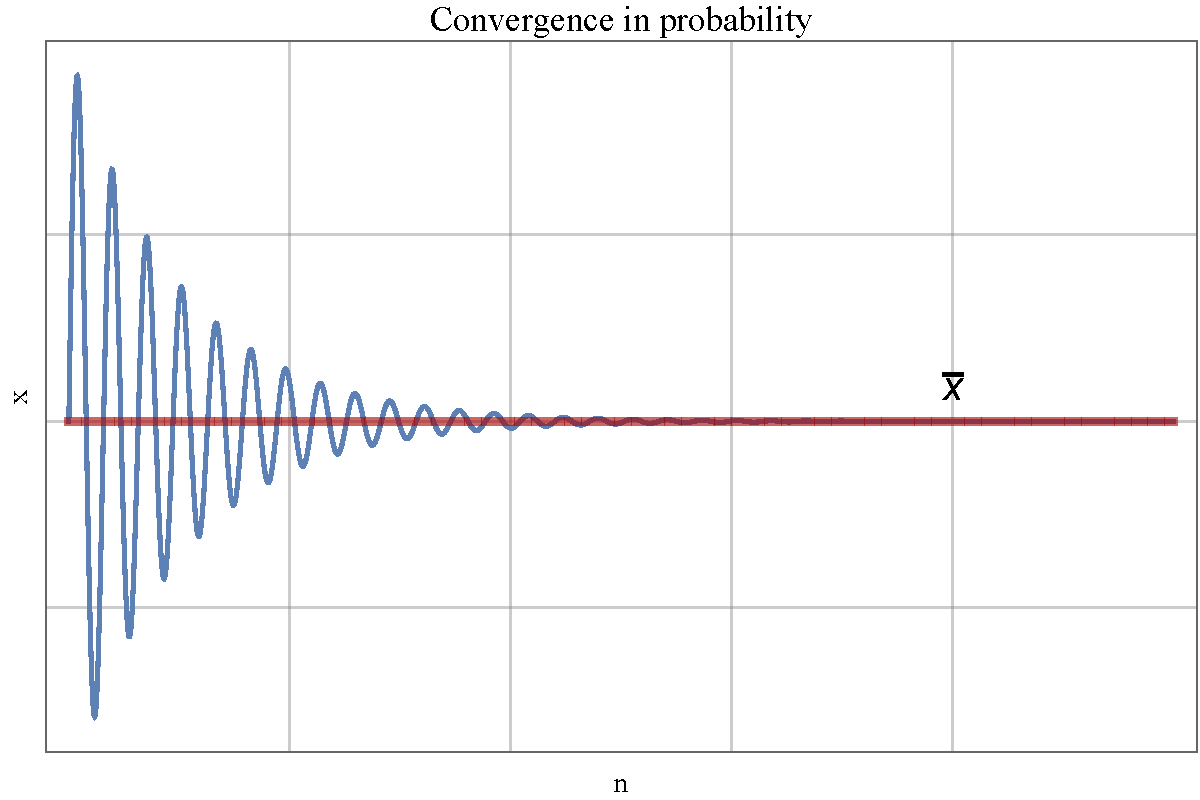
\includegraphics{monte_carlo/convergence.pdf}
	\caption[Convergence in probability.][6pt]{Convergence in probability.}
	\label{fig:convergence}
\end{figure}

\subsection{Law of large number}\index{law of large number}
\label{subsec:law_of_large_number}

Assume to repeat the same measurement $n$ times, where outcome is a random variable $x$ with a given PDF and STD $\sigma$.

The average will be:

\begin{equation}\label{eq:average}
	\bar{x} = \frac{1}{n} \sum_{i = 1}^{n}{x_{i}}
\end{equation}

\begin{itemize}[$\to$]
	\item \newthought{Weak law}\index{law of large number!weak law}: If the mean $\mu$ exists, and if $\lim_{n \to \infty} \left[ \frac{1}{n^{2}} \sum_{i} {\sigma_{i}}^{2} \right] = 0$, then $\bar{x}$ converges to $\mu$ in quadratic mean: $\lim_{n \to \infty} {\mathrm{E}\left[ (\bar{x} - \mu)^{2} \right]} = 0$.
	\item \newthought{Strong law}\index{law of large number!strong law}: If $\lim_{n \to \infty} \left[ \sum_{i} {\left( \frac{\sigma_{i}}{i} \right) }^{2} \right]$ is finite, then $\bar{x}$ converges almost certainly to $\mu$, which means that $P\left(\lim_{n \to \infty} {\bar{x}} = \mu \right) = 1$.
\end{itemize}

\marginnote[-6pt]{Take home message: if the parent mean $\mu$ exists, the more you measure, the closer the sample mean $\bar{x}$ will go to $\mu$.}

\subsection{Central limit theorem}\index{central limit theorem}
\label{subsec:central_limit_theorem}

Recall that if we have a sequence of independent variable $x_{i}$, each with  a distribution with mean $\mu_{i}$ and variance ${\sigma_{i}}^{2}$, the distribution of the sum $s = \sum_{i}{x_{i}}$ will have mean $\mu = \sum_{i}{\mu_{i}}$ and variance $\sigma^{2} = \sum_{i}{{\sigma_{i}}^{2}}$. 

The central limit theorem states that:

\begin{equation}\label{eq:central_limit_theorem}
	\lim_{n \to \infty} {\frac{s - \sum_{i = 1}^{n}{\mu_{i}}}{\sqrt{\sum_{i = 1}^{n}{{\sigma_{i}}^{2}}}} } = \mathrm{Gaus}(0, 1)
\end{equation}

In other words, sum of $n$ random variables tend to a Gaussian.

\marginnote{Or, as Shihong said, “the end of the World is Gaussian”.}

\newthought{Example}: \nameref{exer:gaussian_random_number_generator}.
